\documentclass[a4paper,11pt]{article}
\usepackage{a4wide}
\usepackage[english]{babel}
\usepackage{graphicx}
\usepackage{floatflt}


\begin{document}

\title{Example model:\\Available primitives for development of OpenFLUID functions}
\maketitle


This example is based on a flux model involving 3 simulation functions, 
applied to a spatial domain composed of 13 units distributed into 2 unit classes. 
It aims at showing how values of variables are produced and used in a spatially distributed way.

\bigskip
\bigskip

\section{Overview}

\subsection{Flux model}

\begin{floatingfigure}[right]{7cm}
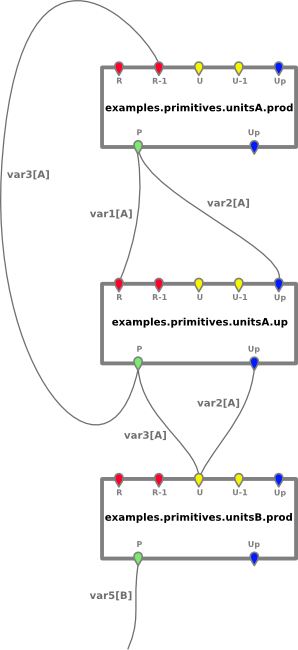
\includegraphics[scale=0.8]{openfluid-engine_example-primitives_en/model.png}
\end{floatingfigure}
The flux model is composed of 3 simulations functions :\\
\begin{itemize}
\item examples.primitives.unitsA.prod
\item examples.primitives.unitsA.up
\item examples.primitives.unitsB.prod
\end{itemize}

\bigskip
\bigskip

The examples.primitives.unitsA.prod function produces values for 
variable var1 and var2 on units of class A, and requires values for var3 on units of class A 
on a previous time step.\\
The examples.primitives.unitsA.up function produces values for variable var3 on units of class A, 
updates values for variable var2 on units of class A, and requires values for var1 on units of class A.\\
The examples.primitives.unitsB.prod function produces values for variable var5 on units of class B,
and requires values for var2 and var3 on units of class A.\\
The flux model is defined in the model.xml file.

\bigskip
\bigskip

\subsection{Spatial domain}

%\begin{floatingfigure}[right]{8cm}
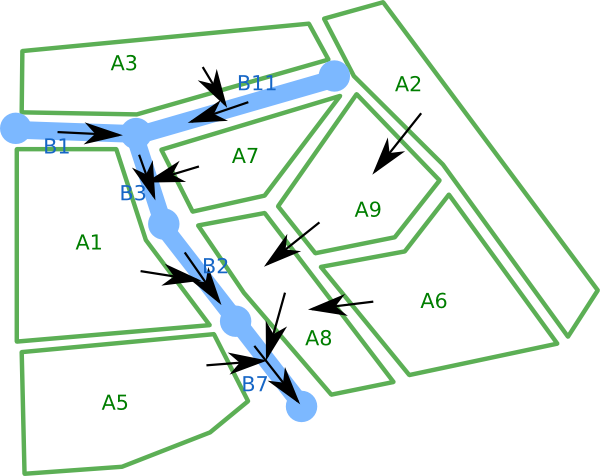
\includegraphics[scale=0.5]{openfluid-engine_example-primitives_en/domain.png}
%\end{floatingfigure}
The spatial domain is composed of 13 units, distributed into 2 unit classes 
(class A and class B). The connections between 
units are defined for each unit independently, as "to" units. The process order 
depends on these connections. This spatial domain is represented as a graph, 
where nodes are units and edges are connections between units.\\
\noindent The spatial domain is defined in *.ddef.xml file(s). 

\bigskip
\bigskip

\subsection{Simulation}

The simulation will run from January 1st, 2001, at 00:00:00 to January 15th, 2001, at 08:01:02.
The fixed time step is 3600 seconds (1 hour). Progressive output is not enabled.\\
\noindent The run configuration is defined in the run.xml file.\\

\bigskip

All variables of all unit classes (A and B) are saved in files. The output configuration is defined in the output.xml file.

\section{Try this example}

\subsection{Build}


\subsection{Run}


\end{document}